
\documentclass[oneside, uplatex]{jsbook}

\usepackage[dvipdfmx]{graphicx}
\usepackage{ascmac}
\usepackage{amsmath}
\usepackage{bm}
\usepackage{mathtools}


\graphicspath{{./figure/}}

\setlength{\textwidth}{\fullwidth}
\setlength{\evensidemargin}{\oddsidemargin}

\title
{
  \vspace{-2cm}
  \vspace{3cm}
  {\huge {\bf Data Analysis Tutorials with Python} }\\
  \vspace{3mm}
  {\bf (Pythonで学ぶデータ解析)} \\
  \vspace{3mm}
  \today\\
  \vspace{6cm}
}
\date{}


\begin{document}

\maketitle
\tableofcontents


\chapter{基本事項}

\section{はじめに}

通常の変数と、確率変数を明確に区別して理解を進めていこう。
ここでいう「通常の」変数とは確率とは無関係に値を持つものであり、例えばその日の体重だったり身長だったり気温だったりするものである。
今日は60kgで、明日はX\%の確率で70kgになる、ということは無いため確率変数ではないと言える。
ただし、解釈によっては体重も確率変数になり得る。
日本人の平均体重を考えると、だいたい60~70kgが標準体重で、数\%の確率で100kgの人がいる、とか。

確率変数は$X$で表され、通常の変数は$x$で表される。

\section{基礎知識}

\subsubsection{平均 $\bar{x}$}

実験の$n$個の測定値($x_1,x_2,...,x_n$)の代表値として、平均は(mean;算術平均または相加平均)がよく用いられる:
\begin{equation}
  \bar{x} = \frac{x_1 + x_2 + ... + x_n}{n}  = \frac{1}{n} \sum_{i=1}^{n} x_i
\end{equation}


\subsubsection{分散 $V$}

各測定値が、平均からどれくらい離れて分布しているか(どれだけばらついているか)を表す指標として分散が用いられる。
分散は平均からのズレ(偏差)の二乗和の平均であり、次のように定義される:
\begin{equation}
  V= \sigma^2 = \frac{1}{n}\sum_{i=1}^{n} (x_{i}-\bar{x})^{2} = \int (x-\bar{x})^2f(x)dx
\end{equation}
平均値の周りにピッタリ分布していれば、 分散は小さくなり、平均値よりも大きかったり小さかったりすると、分散$V$は大きくなる。
また分散の平方根を取ったものを標準偏差$S$という。

\subsubsection{期待値}
ある確率変数$x$に対する期待値は$E[x]$と表され、
\begin{equation}
  E[x] = \sum_{i=1}^{n} x_i p_i 
\end{equation}
と表される。ここで$p_i$は$x_i$を観測する確率である\footnote{サイコロを投げる例であれば、1回投げて$x=$1の目が出る確率は$p=$1/6。}。
$x$が全て等確率で出現するのであれば(ex.理想的なサイコロの例)、
\begin{equation}
  E[x] = \frac{1}{n}\sum_{i=1}^{n} x_i
\end{equation}
と表される。
連続な値を取る確率密度関数に従う場合であれば$x$を観測する確率は$f(x)$と表されるので、
\begin{equation}
  E[x] \coloneqq \int xf(x)dx
  \label{eq:fundamental_concepts:expectation_value}
\end{equation}
と積分形式で表すことができる。

\begin{itembox}[l]{Gaussianの期待値}
  ガウス分布に従う変数の期待値を計算すると:
  \begin{equation}
    E[x] = \int_{-\infty}^{\infty} x \frac{1}{\sqrt{2\pi\sigma}} \exp^{-\frac{(x-\mu)^2}{2\sigma^2} } dx
  \end{equation}
\end{itembox}


確率によって重み付けして平均を計算したもので、
\begin{equation}
  E[x] = \frac{p_1\times x_1+ p_2\times x_2+...+ p_n \times x_n}{n} = \frac{1}{n}\sum_{i=1}^{n} p_ix_i
\end{equation}
重要な性質として、実験結果$x=(x_1,x_2,...,x_n)$の期待値は、
\begin{equation}
  E[x] = \lim_{n\to\infty} = \frac{1}{n}\sum_{i=1}^{n} p_ix_i = \frac{1}{n}\sum_{i=1}^{n} p_ix_i
\end{equation}



\subsubsection{母集団と標本}
ある母集団から確率変数$X$を予想する場合。無限個のサンプル取得が可能であれば、 $X$の平均値(=期待値)は

\begin{equation}
  \mu = \bar{X} = \lim_{n\to\infty} \left(\frac{1}{n} \sum_{i=1}^{n} x_i \right)
\end{equation}

母平均の期待値 $E[\mu]$は、
\begin{equation}
  E[\mu] = \lim_{n\to\infty}\sum_{i=1}^{n}
\end{equation}

で表される。母集団から無限個のサンプルを取得すれば、真の値(母平均)を計算することができることを意味する。
また、母集団の分散(母分散)は

\begin{equation}
  V= \frac{1}{n}\sum_{i=1}^{n} (x_{i}-\mu)^{2}
\end{equation}

で表される。

実際には$n$の値は有限であり、母平均$\mu$や母分散$V$を計算することはできない。
ここで注意が必要である。
\subsubsection{標本分散}
\begin{equation}
  E((X-\bar{X})^2) = \sum_{i=1}^{n} (X_i - \bar{X})^2 = \sum_{i=1}^{n} \left(X_i - \frac{1}{n}\sum_{j=1}^{n} X_j \right)^2
  =
\end{equation}

% ====================================
\section{確率分布}
\subsubsection{ポワソン分布}
\label{subsubsec:poisson}
平均 $\lambda$ 回発生する確率事象が、$x$ 回起こる確率

\begin{table}[h]
  \centering
  \begin{tabular}{lll}
    確率密度関数 & $f(x)=\frac{e^{\lambda}~\lambda^{x}}{x!}$   \\
    期待値      & $E(x)=\lambda$    \\
    分散        & $V(x)=\lambda$
  \end{tabular}
\end{table}

事象が起こる平均値$\lambda$が大きくなるほど、形がガウス分布に近づいていく。
十分に大きくなると$\mu=\lambda$、$V=\lambda$のガウス分布として近似できる。

\begin{figure}[h]
  \centering
  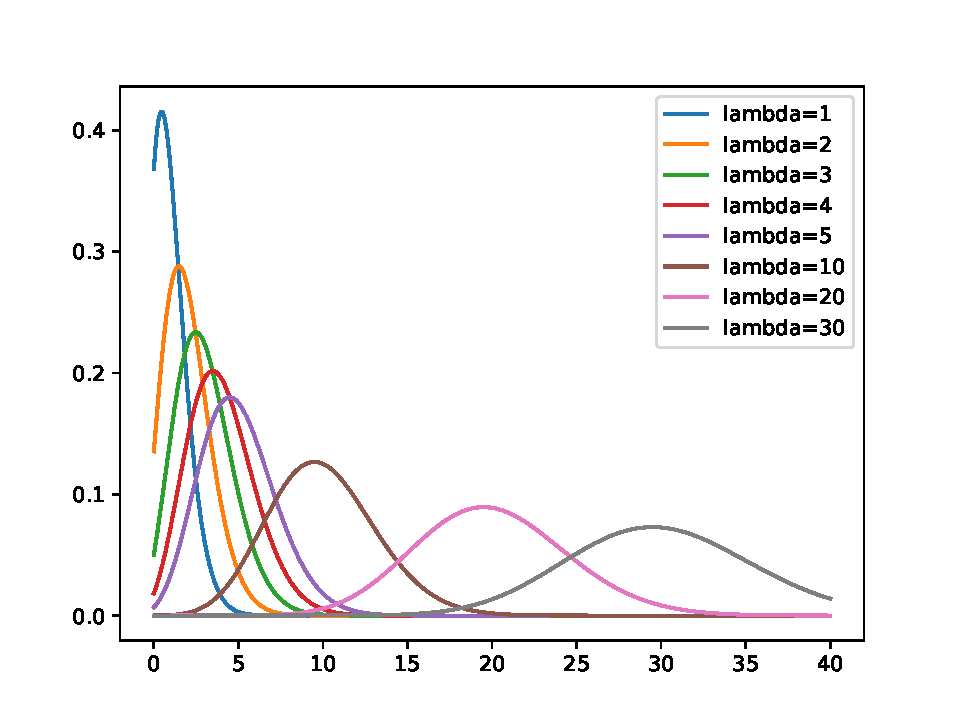
\includegraphics[scale=0.5]{python/poisson_scan.pdf}
  \caption{異なる平均値を取ったときのポワソン分布。平均$\lambda$が大きくなるほど、ガウス分布のような形状になっていくのが分かる。}
\end{figure}

\subsubsection{正規分布(ガウス分布)}

\begin{table}[h]
  \centering
  \begin{tabular}{lll}
    確率密度関数 & $f(x)=\frac{1}{\sqrt{2\pi} \sigma}e^{-\left(\frac{(x-\mu)^2}{2\sigma^2}\right)}$   \\
    期待値      & $E(x)=\mu$    \\
    分散        & $V(x)=\sigma$
  \end{tabular}
\end{table}

\begin{itembox}[l]{ガウス分布の性質その1}
  確率変数$X$が$N(\mu,\sigma^2)$の正規分布に従うなら、$aX+b$は$N(a\mu+b,a^2\sigma^2)$の正規分布に従う
\end{itembox}





% ===================================================== %
\section{共分散}
% ===================================================== %

\subsection{モーメント}
確率密度関数$f(x)$に対して、$x^n$の期待値を定義することができる($n$は整数)。
それらはモーメントと呼ばれ:
\begin{equation}
  a_n \coloneqq E[x^n]
\end{equation}
と定義される。\refeq{eq:fundamental_concepts:expectation_value}より
\begin{equation}
  a_n = \int x^n f(x) dx
\end{equation}
と表される。$n=1$の場合は平均値を表す。

また、$x$が平均値からどれだけ離れているか(散らばっているか)を表す量として中央モーメント
\begin{equation}
  m_n \coloneqq E[(x-\mu)^n]
\end{equation}
が定義されている。
$n=2$は分散として知られている値であり、
\begin{equation}
  m_2 = E[(x-\mu)^2] = \sigma^2 = V[x]
\end{equation}


\subsection{共分散の定義}

確率密度関数が2変数に依存する場合($f(x,y)$)、共分散(covariance)として変数同士の関係性を計算することができる:
\begin{equation}
  \begin{split}
    \mathrm{cov}[x,y]
    & \coloneqq \frac{1}{n} \sum_{i=1}^{n} (x_i-\bar{x})(y_i - \bar{y})  \\
    & = \frac{1}{n} \sum (x_iy_i - x_i\bar{y} - \bar{x}y_i + \bar{x}\bar{y})) \\
    & = \frac{1}{n} \sum x_iy_i - \frac{1}{n}\bar{y} \sum x_i - \frac{1}{n} \bar{x}\sum  y_i + \bar{x}\bar{y} \\
    & = \frac{1}{n} \sum x_iy_i - \frac{1}{n}\bar{y} \sum x_i \\
    & = E[xy] - E[x]E[y]
  \end{split}
\end{equation}
また連続関数を用いると
\begin{equation}
  \mathrm{cov}[x,y] = \int xyf(x,y) dxdy - \int xf(x,y)dx \int yf(x,y)dy
\end{equation}
$f(x,y)=f(x) \cdot f(y)$と表すことができるなら(互いに独立な事象の場合)、
\begin{equation}
  \mathrm{cov}[x,y] = E[xy] - E[x]E[y] = \iint xyf(x)f(y) dxdy - \int xf(x) dx - \int yf(y) dy = 0
\end{equation}
となる。
\ref{fig:fundamental_concepts:covariance}に共分散によるデータの分布の違いを示している。
\begin{figure}
  \centering
  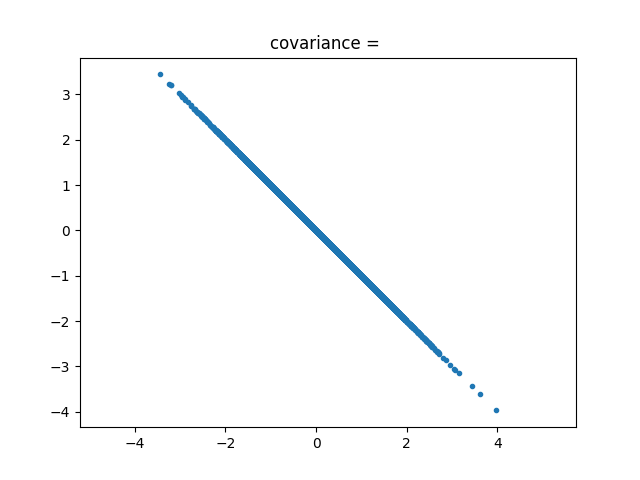
\includegraphics[width=0.3\textwidth]{figure/fundamental_concepts/covariance_-1}
  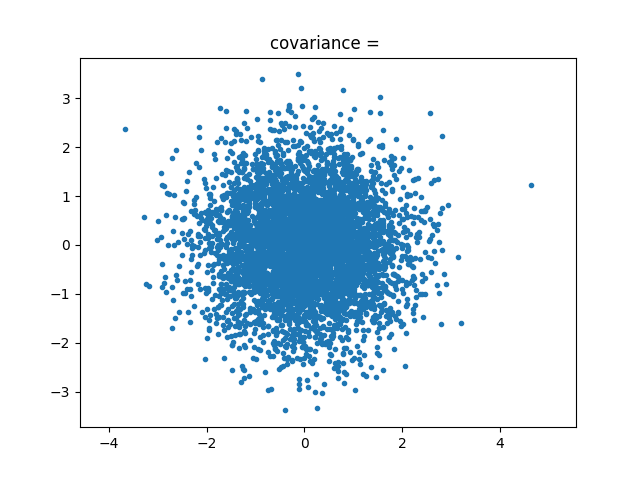
\includegraphics[width=0.3\textwidth]{figure/fundamental_concepts/covariance_0}
  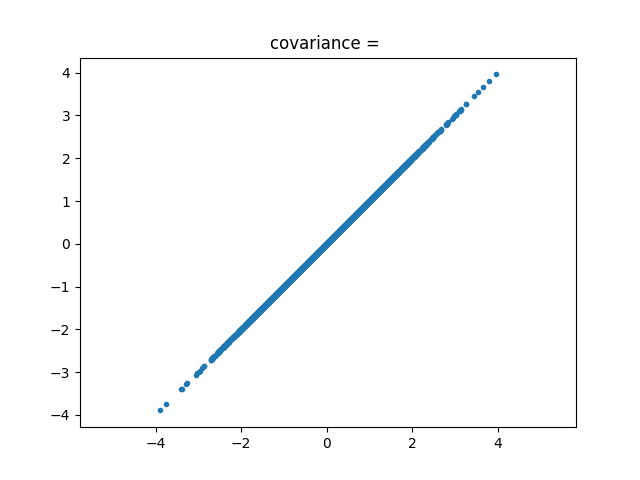
\includegraphics[width=0.3\textwidth]{figure/fundamental_concepts/covariance_1}
  \caption{
    左から順に、cov=-1, 0, +1 の共分散の関係性を持たせてプロットした図。
  }
  \label{fig:fundamental_concepts:covariance}
\end{figure}

また、相関(correlation)として次の量も定義される:
\begin{equation}
  \rho \coloneqq \frac{\mathrm{cov}[x,y]}{\sigma_x\sigma_y}
\end{equation}

これらは多次元への拡張も可能である。
\begin{eqnarray}
  V_{i,j}   &=& \mathrm{cov}[x_i, x_j] = E[x_i x_j] - E[x_i]E[x_j], \\
  \rho_{i,j}&=& \frac{V_{ij}}{\sigma_{i}\sigma_{j}}
\end{eqnarray}


\subsection{共分散行列}


\subsection{多変量正規分布}

Multivariate nominal distribution(多変量正規分布)は:
\begin{equation}
  f(\bm{x}|\mu, \Sigma) = \frac{1}{\sqrt{(2\pi)^N |\Sigma|}} \exp \left( -\frac{1}{2}(\bm{x}-\mu)^T \Sigma^{-1} (\bm{x}-\mu) \right) \coloneqq \mathcal{N}(\mu,\Sigma)
\end{equation}
と定義される。$\bm{x}$は多次元の変数、$\mu$は平均値ベクトル、$\Sigma$は$N\times N$共分散行列、$|\Sigma|$は行列式を表す。




\chapter{検定}

\section{概要}

帰無仮説($H_0$)と対立仮説($H_1$)を用意する。
帰無仮説の元での検定量(test statistics)を、実験結果を元に計算する。
その検定量が$H_0$の棄却領域にいれば、帰無仮説を棄却。棄却領域に入らなければ帰無仮説を採択する。
その判定のために、検定量からp-valueを計算して、棄却領域を定義するp-value($\alpha=0.05$)と比較して棄却領域にいるかどうかを検討すればよい。

$H_0$が棄却されるということは、p-valueがしきい値以下であることを示しており、
これは「帰無仮説が現実世界で正しい仮説であると、めったに起こり得ない結果が本実験結果から得られている」とということであり、
それは帰無仮説が正しい、という仮定が間違っていると考えるのが自然であろう。
そのため棄却されるということである。

ここで重要なことは、どんな量を検定量とするかということと、p-valueを計算するために、検定量の従う分布(sampling distribution)の形が既知であることである。
特にその分布を表式できなければならず、方程式は分かるけれどパラメーターが推測できないということはあまり意味がない。
そこでスチューデントのt-検定やカイ二乗検定が出てくるのである。

\section{カイ自乗検定}

\begin{equation}
  \chi^2 = \frac{(x_1-\mu_1)}{\sigma_1^2} + \frac{(x_2-\mu_2)}{\sigma_2^2} + ... + \frac{(x_n-\mu_n)}{\sigma_n^2} = \sum_{i=1}^{n} \frac{(x_i-\mu_i)}{\sigma_i^2}
\end{equation}

カイ自乗の確率関数

\begin{figure}[h]
  \centering
  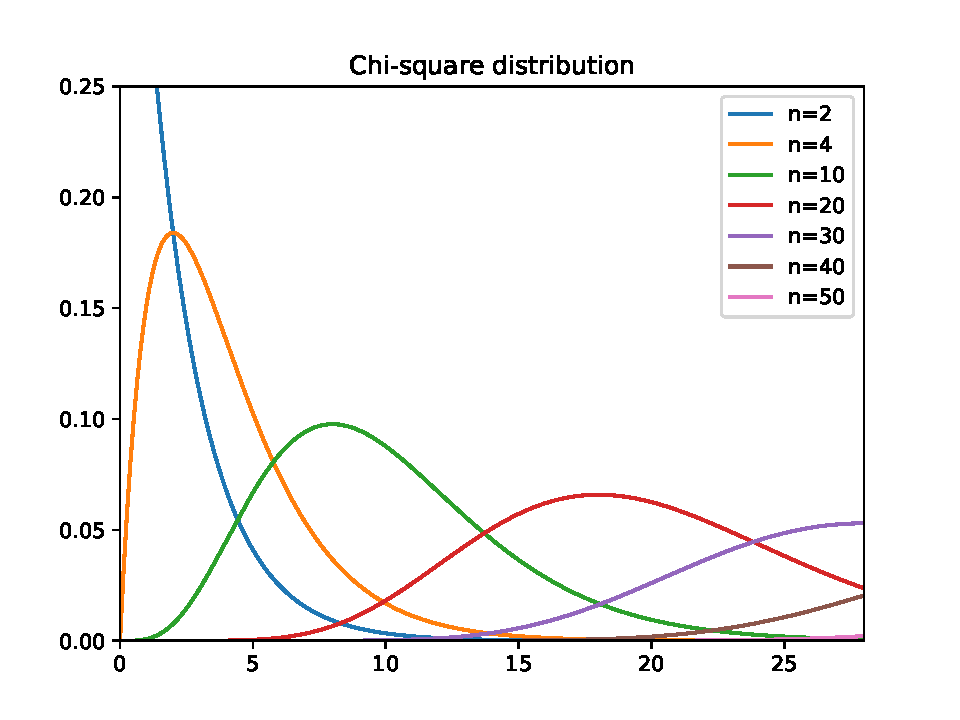
\includegraphics[scale=0.5]{python/ChiSquareDistribution.pdf}
  \caption{$\chi^2$の確率分布。$chi^2$が大きくなるに従って、関数の形が右へシフトしていく。}
\end{figure}


\section{ガウス検定}

検定とは見積もっているパラメーターの真の値について議論する時に用いられる手法である。
例えばガウス分布に従う変数であれば、その真の平均$\mu$と分散$\sigma^2$について知りたいわけである。
しかし実験を何度繰り返しても真の値は絶対に知り得ないわけであるので、実験データから何かを結論づける必要がでてくる。

そこでまず、ガウス分布に従う母集団から無作為に$n$サンプル取り出す試行を考える。
実験データは$\bm{x}={x_1,x_2,...,x_n}$であり、真の値$\mu$と$\sigma^2$を用いると次式の様に標準化できる:
\begin{equation} 
  Z = \frac{x-\mu}{\sigma}
\end{equation}
$Z$は$\mathcal{N}(0,1)$に従う確率変数である。

$Z$はガウス分布に従って様々な値をとるわけであるが、95\%の確率で$[-1.96, 1.96]$の区間に入ることになる。
残り5\%の確率でこの範囲外の値も取り得るが、ほぼ起こらない、と考えてもよい。
以上の議論を少しまとめると、次の様に言い換えることができる。
\begin{itemize}
  \item 「$Z$は$[-1.96, 1.96]$の範囲の値を取る」という条件は95\%の確率で成立する。
\end{itemize}
つまり大体$Z$はこの範囲に存在していると言えるわけである。
ここで、もし仮に$\sigma$が既知であれば、さらに次のように言い換えることができる。
\begin{itemize}
  \item 「$\mu$は$[x-1.96\sigma, x+1.96\sigma]$の範囲の値を取る」という条件は95\%の確率で成立する。
\end{itemize}
ここまできて初めて、真の値$\mu$に対しての条件を引き出せたことになる。

しかし、気をつけなければならないのは、母集団の真の値は大抵全く分からないということである。
上記のような「母平均は分からないけれど、母分散なら分かるよ」というケースはほぼあり得ないのである。
そこで、$\sigma$を何か別の値で置き換えたい気持ちになるが、適当な置き換えをするとそもそも$Z$が従う確率分布が分からなくなり、
結局どんな条件になるか分からなくなってしまう。
そこで登場するのが次節で議論するスチューデント分布である。
このスチューデント分布は、分散の置き換えの指標を示し、また置き換えた後の$Z$が従う確率分布を記述することができる(=存在区間に対する条件を書き出せる)。


\section{スチューデント検定}

\subsection{検定における確率の解釈}

スチューデント分布の$t$は次のように示される:
\begin{equation}
  t = \frac{\hat{x}-\mu}{\sqrt{\frac{s^2}{n}}}
\end{equation}
ここで$\mu$は$x$の母集団の平均、$s$は不偏分散($\sigma$ではない)である。
この関係式を用いることで母平均に対しての条件を考えることができる、というのがスチューデント検定の概要である。
このときに、よく考えないと誤った解釈をしてしまう箇所がある。

$t$が$1-\alpha$の確率で含まれる区間を$[a, b]$で定義する。
確率変数は$t$(正確には$t$の中の$x$)であることに留意すると、次の言い換えが成り立つことが分かる。
$a<t<b$は95\%の確率で成り立つ。

しかし、確率変数は$t$であり、区間$[a,b]$は確率変数でないので、次の言い換えは成り立たないことが分かる。
「$[a,b]$は95\%の確率で$t$を含む」区間は定数であるので、実際の観測値$t$を含むかどうかは確率ではなく「含むor含まない」の2択でしかない。
ここで気をつけなければならないのは、いま着目している確率変数が何か、である。

スチューデント検定では、次のような不等式変形を行う。

\begin{eqnarray}
  a < t = \frac{\hat{x}-\mu}{\sqrt{\frac{s^2}{n}}} < b \\
  \hat{x} - b \sqrt{\frac{s^2}{n}} < \mu < \hat{x} - a \sqrt{\frac{s^2}{n}}
\end{eqnarray}

そのため、次のような誤った解釈が頭に浮かぶ。
「$\mu$は95\%の確率で、区間$[\hat{x} - b \sqrt{\frac{s^2}{n}}, \hat{x} - a \sqrt{\frac{s^2}{n}}]$に含まれる」。しかし、先程の留意事項を思い出せば、
母平均$\mu$は確率変数ではなく、ある決まった(と言っても未知ではあるが)値の定数である。
そのためこの文言は成り立たない。
確率変数はどこまで行っても$t$もしくは$\hat{x}$であるので、正しくは、
「区間$[\hat{x} - b \sqrt{\frac{s^2}{n}}, \hat{x} - a \sqrt{\frac{s^2}{n}}]$は95\%の確率で母平均$\mu$」を含む。である。













\chapter{誤差論}
\subsection{誤差の伝播}
N点の計測($x_1, x_2, ..., x_n$)を行う。測定値それぞれに誤差がついている場合($x_1\pm\Delta x_1, x_2\pm\Delta x_2, ..., x_n\pm\Delta x_n$)、測定結果の合計、平均にはどのような誤差が付くか。


\subsubsection{加減乗除}

\begin{eqnarray}
  (x\pm \sigma_x) \pm ( y \pm \sigma_y) &=& (x\pm y) \pm \sqrt{ \sigma_x^2 + \sigma_y^2} \\
  (x\pm \sigma_x) / ( y \pm \sigma_y)   &=& \frac{x}{y} \pm \sqrt{ \left( \frac{\sigma_x}{y} \right)^2 + \left( \frac{x \cdot \sigma_y}{ y^2} \right)^2}
\end{eqnarray}



\subsubsection{合計の誤差}

\begin{equation}
  y=\Sigma_i~x_i=x_1+x_2+...+x_n=n\times\frac{1}{n}(x_1+x_2+...+x_n)=n\bar{x}
\end{equation}

誤差の和はyに対して、

\begin{equation}
  \Delta y = \sqrt{\left(\frac{\partial}{\partial x_1}y \right)^2 \Delta x_1^2 + ... + } = \sqrt{\Sigma_{i=1}\left(\frac{dy}{dx_i}\right)^2\Delta x_i^2}
\end{equation}

として伝搬する(誤差伝搬の公式).
今の場合、
\begin{equation}
  \frac{\partial}{\partial x_1}n\times \frac{1}{n}(x_1+x_2+...+x_n)=1
\end{equation}

となるので、

\begin{equation}
  \Delta y=\sqrt(\Sigma(\Delta x_i)^2)
\end{equation}

測定値$x_{i}$の分散は、測定したn点から事前に計算される。
なので誤差の伝播の式を進めると、
\begin{equation}
  \Delta y=\sqrt{ns^2}=\sqrt{n}s
\end{equation}
となる。

\subsubsection{平均の誤差}
測定値の平均値には、
\begin{equation}
  \bar{x}=\frac{1}{n}\Sigma x_i
\end{equation}

誤差伝搬の式を適用して、
\begin{equation}
  \Delta \bar{x} = \sqrt{n\times\left(\frac{1}{n}\right)^2s^2}=\frac{1}{\sqrt{n}}
\end{equation}

この式は、平均値の誤差は測定点の数のルートN倍で小さくなっていくことを示している。測定を繰り返し行い、平均を得た場合にどのように誤差が小さくなっていくかを示している。

- 計数の誤差
- 計数$N$の統計誤差は$\sqrt{N}$で表される

\subsubsection{ヒストグラムにおける誤差}
ここまでの議論は、例えば粒子の不変質量を測定した場合に、あるイベントでは$m_1$[GeV]、あるイベントでは$m_2$[GeV]、...と測定した時に、その測定量に対してどれくらい誤差が付いているかを論じてきた。
議論をもう一度繰り返すと、$n$回測定した質量の平均値は、

\begin{equation}
  \bar{m}=\frac{1}{n}\Sigma m_i
\end{equation}

測定結果の分散は、

\begin{equation}
  V=\Sigma(m_i-\bar{\mu})・・・(☆)
\end{equation}

で表される。しかし、これらの議論はヒストグラムの場合には少し特殊な議論となる。よく不変質量の分布をヒストグラムにしたりして議論を進めていくが、この時によく「ヒストグラムにエラーバーを付けて」と言われるが、このエラーバーはここまでの誤差とは若干違っている。(☆)の誤差は不変質量の測定値に付くものであって、ヒストグラムのそれぞれのビンにつくものではない。

\subsection{ビンにつく誤差}
「ヒストグラムのエラー」は、そのビンにいる統計数に対して考える。よくみるヒッグス粒子の不変質量を例に取ってみよう。(☆)の議論はヒッグス質量125GeVに対して$125GeV \pm \sigma_{H}$ という形で付くものである。これは強いて言うなら下図の横方向(x軸方向)に対しての誤差である、

では、図に示されている縦方向の誤差は一体なんでしょうか?これこそが高エネ実験領域でよく耳にする「統計誤差」というものである。

\subsubsection{考え方}
例えば1番目のビンに注目する。このビンでカウントされている事象数を仮に460事象と読み取ることにする。
これを「とある確率分布に従う事象を観測し、平均値460事象観測した」と捉える。よく用いられる確率分布はポワソン分布である(\ref{subsubsec:poisson}節)。
簡単に分散$V=460$、$\sigma=\sqrt{460}$と求めることができる。これがヒストグラムの計量の際の誤差である。感覚的には、縦方向に(各ビンに)ある確率分布があって、それらの平均値をつなぐようにしてヒッグス質量分布が計算されているとすればいい。

\subsubsection{誤差はどうなっていくか}
統計量が溜まってくると、1ビン〜10000事象とかがあるかもしれない。こういうときにポワソン分布でヒストグラムのエラーバーを考えていいのか?という疑問が湧いてくる。答えは**ガウス分布**を使う、が、「考え方」は変わらないということである。

- 二項分布→ポワソン分布
- 二項分布において$\lambda$を一定にして、$n$を大きく、$p$を小さくするとポワソン分布になる
- ポワソン分布→ガウス分布
- ポワソン分布で$\lambda$を大きくすると、期待値$\lambda$、分散$\lambda$のガウス分布になる
- 二項分布→ガウス分布
- 期待値$np$、分散$np(1-p)$の両方が大きい場合、期待値$np$、$分散np(1-p)$のガウス分布になる

上記の関係性を思い出せば、1ビンあたりの統計量(=1ビンで観測したイベントの期待数)が大きくなっても、結局は分散$\lambda$のガウス分布に従っているので、ヒストグラムのエラーバーはやはり$\sqrt{N}$になる。

つまりヒストグラムのエラーバーは、

$N\pm\sqrt{N}$

の関係で成り立っている(ポワソン分布orガウス分布に由来するものであることに留意)。


\subsection{「誤差は$\frac{1}{\sqrt{N}}$で小さくなっていく」の真実}
誤差の大きさそのものが$\frac{1}{\sqrt{N}}$なのではなく、ここで言っている誤差は「XX\%」の誤差に相当するものである。ヒストグラムの誤差は、

\begin{equation}
  N\pm\sqrt{N}
\end{equation}

で付くものだったから、1ビンに対する誤差は

\begin{equation}
  \frac{\sqrt{N}}{N}\times 100 = \frac{1}{\sqrt{N}} \%
\end{equation}

である。つまり、1ビンに入る統計数が多くなればなるほど、統計量が増えれば増えるほど、誤差は、$\frac{1}{\sqrt{N}}$で小さくなっていきます。
なので、できる限り統計量を貯める、という至極まっとうな感想が生まれてきます。

ちなみに、例えばあるビンの統計数が1事象だった場合の誤差は、

\begin{equation}
  1\pm 1
\end{equation}

で、「なんだ、誤差の大きさは1じゃん、小さいじゃん」と思うかもしれないが、

\begin{equation}
  \frac{\sqrt{1}}{1}\times 100 = 100 \%
\end{equation}

の誤差が付いているという事実を忘れてはならない。ちなみに100事象貯めれば、

\begin{equation}
  \frac{\sqrt{100}}{100}\times 100 = 10 \%
\end{equation}

10\%の誤差にまで削減することができるのである。




\chapter{RooFitで学ぶ統計処理}
https://twiki.cern.ch/twiki/bin/view/Main/LearningRoostats
\section{ジャーゴン}
\begin{itemize}
  \item フロートにする:定数として扱わないこと。MLEの時に、何を変数として扱って、何を定数として固定するかに関する話題でよく出る。setConstant(0);
\end{itemize}
\section{関数}




\chapter{HistFactory}
RooFitやRooStatで処理を行っていくためには、RooWorkspaceを作成する必要がある。
簡単なチュートリアルレベルであればRooWorkspaceの作成は簡単な作業であるが、実際の解析ではかなり骨の折れる作業である。
そこでHistFactoryと呼ばれるパッケージがROOTでは提供されていて、これを用いることでユーザーは自分のヒストグラムから簡単にRooWorkspace(=確率密度関数)を計算して保存することができる。

\section{使い方}
ROOTにはhist2workspaceというコマンドが用意されていて\footnote{ローカルでROOTを触っている人はインストールしていないかもしれない。ROOTを自分の環境でビルドしたときのことを思い出しましょう。}、これに「どのヒストグラムをどういう設定で使用するか」を記したXMLファイルを食わせることでRooWorkspaceがアウトプットされる。

\section{marked Poisson model}
marked poisson modelと呼ばれる確率密度関数をヒストグラムの情報から計算する。
ヒストグラムのビンの情報はシグナル数$S$と背景事象数$B$との間に次の関係を定義する。
$\nu_{b}^{sig}$は着目する$b$番目のビンに含まれるイベント数で、次の等式が成り立つ(単にビンを端から端まで足し合わせたら全イベント数になるということを言っている)。
\begin{equation}
  S = \sum_{b} \nu_{b}^{sig}
\end{equation}
\begin{equation}
  B = \sum_{b} \nu_{b}^{bkg}
\end{equation}

シグナルと背景事象の"shape"は$f_S(x_e)$、$f_B(x_e)$で表現する。
ヒストグラムをhist->Scale(1/hist->Integral())することと等しく、そのイベントがどのような確率で出現するかを表すことができる。
\begin{equation}
  f_S(x_e) = \frac{\nu_{be}^{sig}}{S\Delta_{be}}
\end{equation}

\begin{equation}
  f_B(x_e) = \frac{\nu_{be}^{bkg}}{S\Delta_{b_e}}
\end{equation}
以上の定義した式を用いて次のmarked poisson modelを計算する。
\begin{equation}
  P({x_1,..,x_n}|\mu) = \mathrm{Pois}(n|\mu S+B) \left[ \prod_{e=1}^{n}\frac{\mu Sf_S(x_e)+Bf_B(x_e)}{\mu S+B} \right]
\end{equation}
この式は、イベント数やその他のパラメータが固定(観測からわかっていれば)であれば、$\mu$にのみ依存し、これはまさしくLikelihoodを表している。

\section{HistFactoryのレンプレート}
はじめに使用する添字について簡単な説明を行う。
\begin{itemize}
  \item e:イベント
  \item b:ビン
  \item c:チャンネル
  \item s:サンプル
  \item p:パラメーター
\end{itemize}

さらに、
\begin{itemize}
  \item ${\phi_p}$:パラメーター毎の規格化定数(NormFactor)
  \item ${\alpha_p}$:系統誤差に関連するパラメーター、それ自身は事前にCR等で見積もっておくもの(OverallSys, HistoSys)
  \item ${\gamma_{csb}}$:ビンごとの系統誤差(ShapeSys、)
\end{itemize}
を定義する。 実際にHistFactoryが計算する数式は次のものである。
\begin{equation}
  P(n_c,x_e,a_p|\phi_p,\alpha_p,\gamma_b) = \prod_{c}\left[\mathrm{Pois}(n_c|\nu_c) \prod_{e=1}^{n_c}f_c(x_e|\alpha) \right]
  \times G(L_0|\lambda,\Delta_L)
  \times \prod_{p} f_p(a_p|\alpha_p)
\end{equation}




\chapter{Pythonと学ぶ統計}
\section{最小二乗法 (least square)}
python/chi\_square.py
$N$組のデータ$(x_i,y_i)$を測定した($i=1,...,N$)。これらを尤もらしく表すことができる関数$y=f(x)$を求めたい。
想定する状況は、実験者が$x_i$を固定して、$y_i$を測定していく、というもの。
各$y_i$はとある平均値の周りにふらつきを持って測定される。以下では簡単に線形近似の場合を考える。
\begin{equation}
  y = ax + b
\end{equation}
の係数を実験データから求めたい。そこで次のような値を考える。

\begin{equation}
  \Phi(a,b) = \sum_{i=1}^{N} w_i r_i^{2} = \sum_{i=1}^{n} w_i[f(x_i)-y_i]^2
\end{equation}

$r_i$は残差(residual)と呼ばれる値であり、データ点とモデル曲線との差を表している。
$w_i$は各データ点に対する重みであり、分散の逆数に比例した値を持つ。
仮に$w_i$が$1/\sigma_i^2$に全く等しい場合、$\Phi$は$\chi^2$に等しくなるため、最小二乗フィットはカイ自乗フィットとも呼ばれる。


誤差を含むような実験データ値から、もっともらしい関数の形を決定する時に用いられる手法。
$n$個のデータ点$(x_1,y_1), (x_2,y_2), ... (x_n, y_n)$をフィットする際に(関数の形は経験的に決定する)指標として用いる。



% ----------------------------------------- %
\chapter{統計処理の応用;高エネルギー実験}
% ----------------------------------------- %

高エネルギー素粒子実験では、未知の素粒子の兆候を掴むために様々な測定を行っている。
新しい物理模型が存在すればこの様な兆候として発見することができる、という事前の調査に基づいて研究を進めていく。
信号事象として新粒子の兆候、背景事象として既存の理論に起因する兆候を割り当てて考えていくことが多い。
新粒子の発見が勿論究極の目標であるが、そこに至るまでの過程で様々な理論模型を棄却して可能性のある領域を絞っていく作業も
非常に重要である。
高エネルギー実験ではこれらを統計処理で発見・棄却の評価を行っていくが、通常の検定とは少し毛色が異なるため独立した章として、
本章でその概要と詳細について議論する。

\section{はじめに}

高エネルギー実験では仮定する新物理事象から予測される兆候を掴むために、粒子のエネルギーや角度情報を測定する。
例えばヒッグス粒子であれば、粒子の不変質量を計算することで($H\to \gamma\gamma$などの反応)125GeV付近にピークを持つ不変質量分布を観測することができる。
また、ヒッグス粒子の反応とは全く関係のない2光子で不変質量を組んでしまうことも予想される。
そのため、得られる不変質量分布としては背景事象(ここでは標準理論で予想される通常の反応過程)の分布の上に、ピークが乗った様なヒストグラムを描くことができる。
実験屋としては、そのピークの幅(分解能)を絞るための手法の開発・改良を行ったり、背景事象をいかに削減するか・信号事象を
いかに無駄なく取得するかに工夫を凝らしていく。
そのうえでピークが見つかれば「発見」という結論となる。

問題は、背景事象から計算した分布が偶然125GeVにピークを持っただけではないのか、等どのような確率の上に成り立っていることであるかを
評価していく必要がある。

素粒子実験では目当ての事象をカウントして、そのカウント数$s$で理論モデルの検証を行っていく。
その際には背景事象もあるカウント数$b$だけ含まれてしまうことから、たとえ信号事象を観測できたとしてもノイズに埋もれてしまったら発見にはつながらない。
そこで、最終的には$b$に対して$s$が優位に大きいかどうかを議論する必要があるのだが、この手法にはいくつかの種類があり

\begin{itemize}
  \item カウンティング
  \item シェイプフィット
\end{itemize}

が主な手法である。大層な名前がついているが特に難しいわけではないのでじっくり考えれば理解できるはず。
信号の発見を行うには、$s=0$の仮説の$p-value$を計算することが一般的である。

これは、目的の新物理は世の中に存在しない場合($s=0$)に、実験で得られたイベント数がどれくらい普通に起きるかの目安となる。

\section{検定について}

\ref{}で述べた検定について、再度確認を行う。
ここでは帰無仮説$H_0$として「信号事象は存在する」を選択し、対立仮説として「信号事象は存在しない、背景事象で世の中は記述される」
を選択する。
しかし帰無仮説が棄却されたからといって、直ちに仮定する信号事象が存在する、という結論にはならない。

\section{p-value}

\begin{equation}
  p = \int_{\alpha}^{\infty} f(x)dx
\end{equation}

例えばガウス分布であれば、p値が小さければ小さいほど起こり得ない事象であると理解できる。
高エネ業界では専ら、p値を標準化された正規分布におけるsignificance $Z$ に焼き直して議論する。
\begin{equation}
  Z = \Phi^{-1}(1-p)
\end{equation}
$p=0.5$のときに$Z=0$、$p=0.05$のときに$Z=1.64$、$p=2.9\times 10^{-7}$の時$Z=5$となる。
つまり、標準化された正規分布の平均値から何$\sigma$離れた場所に位置しているかの指標となる。

\section{$S/\sqrt{B}$の導出}
背景事象$B$に対して信号事象$S$がどれだけ優位に多いかを表す指標であり、発見感度の議論の仕方としては最も基本的なものの一つである。
ポワソン分布の平均値$\lambda$が大きいときにガウス分布で近似できる性質を使う。
素粒子実験においてポワソン分布の平均値とは、「実験で観測できるとされる事象数 $s+b$」を意味する。
ゆえに十分な統計を溜めることのできる実験では以下の近似式を用いることができる。

\begin{equation}
  f(x)
  = \frac{1}{\sqrt{2\pi}\sigma} e^{\frac{(x-\mu)^2}{2\sigma^2}}
  = \frac{1}{\sqrt{2\pi(s+b)}} e^{\frac{{x-(s+b)}^2}{2(s+b)^2}}
\end{equation}

ここでポワソン分布は、 $\mu = s+b$、$\sigma = \sqrt{s+b}$
のパラメータを持つガウス分布で記述されている。

この近似式を用いた場合に、信号事象がゼロの仮説(background only hypothesis)に対するp値は次のように計算できる($s=0$)。

\begin{equation}
  p = 1 - \Phi \left(\frac{x-\mu}{\sigma} \right) = 1 - \Phi \left(\frac{x-b}{\sqrt{b}} \right)
\end{equation}

ここから、予想されるsignificance を求めることができて、
\begin{equation}
  \Phi \left(\frac{x-b}{\sqrt{b}} \right) = 1-p \\
\end{equation}

\begin{equation}\label{eq:signigicance_Z}
  \frac{x-b}{\sqrt{b}} = \Phi^{-1} (1-p) = Z
\end{equation}

(\ref{eq:signigicance_Z})式より、$x=s+b$の場合に予想されるsiginificanceは、

\begin{equation}
  \mathrm{med}[Z|s] = \frac{s}{\sqrt{b}}
\end{equation}

この式は信号事象の優位性を議論する時に広く用いられているものである。

\begin{figure}[h]
  \centering
  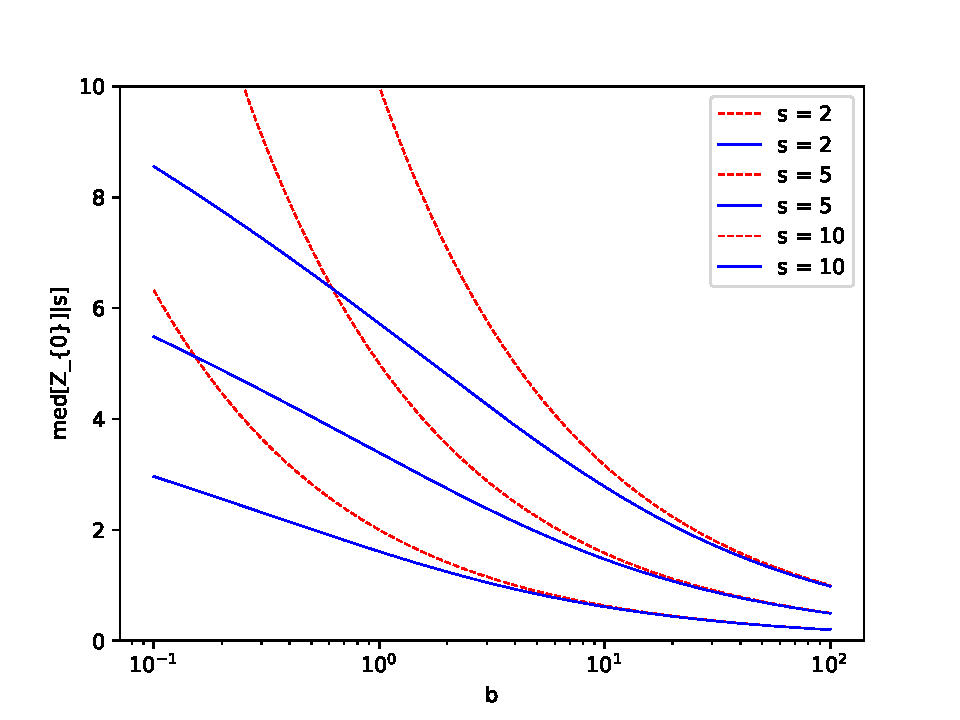
\includegraphics[scale=0.8]{python/discovery_significance.pdf}
  \caption{予想されるsiginificanceの分布。
  赤線は$Z=s/\sqrt{b}$、青線は$Z=\sqrt{2\left((s+b)\log\left({1+\frac{s}{b}}\right)-s\right)}$から見積もった曲線。
  Asimov siginificanceの方が背景事象が少なくなってくる領域でも正しくexpected limitを見積もることが可能である。
  基本的には$s/\sqrt{b}$はそのような領域ではoverestimationになっているだけで、$s/\sqrt{b}$同士で比較する分には多少の意味はある。
  }
\end{figure}


\section{Statistical test}

\begin{equation}
  \lambda(s) = \frac{L(s,\hat{\hat{\theta}}(s))}{L(\hat{s},\hat{\theta})}
\end{equation}


\section{Asymptotic formulae}
\subsection{導入}
ある確率変数$x$を測定して$N$ビンのヒストグラムを作成した($n_1,n_2,...,n_N$)。
$i$番目のビン内のイベント数の期待値は次のように表される。
\begin{equation}
E[n_i] = \mu s_i + b_i
\end{equation}
ここで$s_i$と$b_i$は$i$番目のビンにおける信号数と背景事象数の平均値である。
\begin{eqnarray}
 s_i = s_{tot}\int_{\mathrm{bin}~i}f_s(x;\theta_s)dx \\
 b_i = b_{tot}\int_{\mathrm{bin}~i}f_b(x;\theta_b)dx
\end{eqnarray}
$f(x;\theta)$は各モデルの確率密度関数を表しており、積分することで注目するビンに事象が得られる確率を計算することができる。また、$\mu$は信号強度であり、$\mu=0$の時にはbacground only hypothesis、$\mu=1$のときには信号を含んだ仮説を表現することができる。
$\theta$は確率密度関数の形状を決めるパラメーターで、$(\theta_s,\theta_b,b_{tot})$をまとめてnuisance parameter として扱う。

\subsection{likelihood}
作成したヒストグラムに対する尤度関数は、とあるビンに事象が観測される確率(ポワソン分布)の積で表すことができる。
\begin{equation}
    L(\mu, \theta) = \Pi_{\j=1}^{N} \frac{(\mu s_j + b_j)^{n_j}}{n_j!}e^{-(\mu s_j + b_j)}
\end{equation}
さらに、control regionを定義した解析では、CRにおける尤度関数も式に含めることができる。

\subsection{Profile likelihood ratio}
信号強度$\mu$を試験するために、profile likelihood ratio $\lambda(\mu)$を用いる。
\begin{equation}
  \lambda(\mu) = \frac{L(\mu,\hat{\hat{\theta}})}{L(\hat{\mu},\hat{\theta})}
\end{equation}
分母はLikelihoodの最大値、分子は$\mu$をとある値に固定した時にLikelihoodが最大となるように求めた$\theta$を用いたときの値。
尤度関数を最大にするパラメータの組み合わせは$(\hat{\mu},\hat{\theta})$であるため、常に分子は分母より小さいか分母に等しくなるので、$0<\lambda<1$が成り立つ。
$\lambda=1$はデータと$\mu$がよく一致することを表していて、0に近づくほど実験データと乖離している($\mu$を仮定した理論では実験データを説明できない、棄却される対象となる)ことが表される。

\subsection{test statistic $t_\mu=-2\ln\lambda$}
statistical testを行う際には、$\lambda$をさらに次の様に変換して用いることが多い。
\begin{equation}
  t_\mu=-2\ln\lambda(\mu) = -2 \left(\ln L(\mu,\hat{\hat{\theta}}) -  L(\hat{\mu},\hat{\theta} ) \right)
\end{equation}
先程の$\lambda$の範囲の議論より、$t_\mu$は$-2<t_\mu<0$の範囲を動く。
よって0に近いほど(値が大きくなるほど)、データと$\mu$の整合性が取れないことを表している。
\begin{equation}
p_\mu = \int_{t_{\mu,obs}} ^{\infty} f(t_\mu|\mu) dt_\mu
\end{equation}
$t_{\mu,obs}$は実験データから見積もった値、$f(t_\mu|\mu)$は$t_\mu$が得られる確率密度関数を表している。

\subsection{Test statistics $t_\mu$ for $\mu > 0$}
一般的に信号モデルは、既存のモデルに対してさらに数イベント信号が観測できると予測する。
そのため信号強度は正の値をとる。その場合を試験量も記述しておく。$\mu>0$の領域では今まで通りのlikelihood ratioを用いて、0以下の領域では$\mu$の値を0に固定したlikelihood ratioを定義しておく。

\subsection{Test statistics $q_\mu,q_0$}
高エネ実験では新物理$\mu=1$を探している。
実際の統計処理では$\mu=0$のbackground only hypothesisを棄却する方向で計算を進めていく\footnote{ここが少し混乱の元。示したいのは信号を含んだモデルが存在することであるが、統計処理では「信号を含まないモデル$H_0$では実験データを説明できない$\to$新しいモデルが必要となる」というロジックで進んでいく。}。
よって方針は、$\mu=0$のtest statisticsを正しく評価していくこととなる。
(で、問題は)ここから定義した$t_\mu$をさらにいろいろ条件を変えたときの式として、$q_\mu$に置き換えて議論していくので、本書もそれに倣う\footnote{
式の形は$t_\mu$の議論の時に示したとおりだが、$q_\mu$と明記したときには「$\mu$の値に関して条件を掛けて立式していきますよ」という意思表示だと思ってもらえればいい。}。

\begin{equation}
  q_0 = -2\ln\lambda(0) : \hat{\mu} > 0
\end{equation}
\begin{equation}
  q_0 = 0 : \hat{\mu} < 0
\end{equation}

\begin{equation}
  q_\mu = -2\ln\lambda(\mu) : \hat{\mu} < \mu
\end{equation}
\begin{equation}
  q_\mu = 0 : \hat{\mu} > \mu
\end{equation}

\section{Profile likelihood ratio の近似式}
信号強度$\mu$を試験する場合を考え、データ点は$\mu'$に従って分布しているとする。
\begin{equation}
-2\ln\lambda(\mu) = \frac{(\mu-\hat{\mu})^2}{\sigma^2} + O(1/\sqrt{N})
\end{equation}
ここで、$\hat{\mu}$はmean $\mu'$、標準偏差$\sigma$のガウス分布に従う。$N$はサンプル数を表す。
$\sigma$は共分散から簡単に求めることができて、
\begin{equation}
  V_{ij} = \mathrm{cov}[\hat{\theta_i}, \hat{\theta_j}]
\end{equation}

\section{カウンティング(1ビンフィット)}
ポワソン分布に従う事象を$n$事象観測して、1ビンのヒストグラムで評価する場合を考える。
SRにおける期待値は
\begin{equation}
E[n] = \mu s + b
\end{equation}
$s$は信号モデルから予想される信号事象数の平均値、$b$は背景事象数の期待値、$\mu$は信号強度を表す。
$b$はnuisance parameter \footnote{nuisanceとは迷惑なこと、厄介なこと、の意味を持つ単語。高エネの人が真に興味があるのは信号数なので、まぁ背景事象数は邪魔だということか。}であり、CRにおける背景事象数の分布から制限をかけることができる。
CRにおける背景事象の期待値は、SRとCRにおける背景数の違いを表す scale factor を$\tau$で表すと、
\begin{equation}
E[m] = \tau b
\end{equation}
と記述することができる。
実際の解析ではこの$\tau$もnuisance parameterとしてフィットから求める手順を踏むが、
ここでは簡単のために既知の値として話を進める。

実験から得られる値はSRの事象数$n$、CRにおける自少数$m$、興味のあるパラメータ(parameter of intereset; POI)$\mu$、そしてnuisance parameter $b$である。
ポワソン分布に従うような場合に、$\mu$と$b$に対して実験結果から次のような尤度関数を定義することができる。


\section{シェイプフィット}
1ビンではなく、分布の形を反映した統計処理を行いたい場合、こちらの手法を用いる。
俗語的に
\begin{itemize}
  \item シェイプフィット
  \item シェイプでフィットした
\end{itemize}
とか呼ばれる。

\section{CLs法}
以下で定義する$CL_s$と呼ばれる量をtest statisticとして用いて解析感度を評価する手法。

\begin{equation}
CL_s = \frac{CL_{s+b}}{CL_b}
\end{equation}

$CL_{x}$はたどっていくと$\mu$に依存する。
よく用いられるのは95$\%$CLsであり、$CL_s=0.05$となる$\mu$の値を探してそれを$\mu_{up}$として
解釈し、最終的に断面積の上限値設定に使用する手法である。


\chapter{高エネルギー実験における統計処理}

\section{Likelihood}
私達が興味のあるパラメータは(究極的には)信号事象の数に相当する信号強度$\mu$である。
自然界では既に$\mu$は定まった値を持っており、それを人間が知らないだけである。
そのため実験データが得られる確率は
\begin{equation}
P(\rm{data}|\mu)
\end{equation}
と表すことができる。
実験屋が持っている情報は実験データ(とシミュレーションサンプル)であり、データから確率密度関数を求める必要がある。
これがLikelihoodの意味するところである。
\begin{equation}
L(\mu)
\end{equation}

Likelihood 関数を用いると、信号強度$\mu$の推定も最大尤度法(Maximum likelihood; ML)を用いることで可能となる。
慣習的に推定量はハット記号で表し

\begin{equation}
\hat{\mu} = arg max L(\mu)
\end{equation}

と信号強度を推定することができる。
統計量が増加すると $\hat{\mu}\to\mu^{\rm{truth}}$ に近づく。

\subsection{Likelihoodを計算する}
実際の実験では例えば質量の分布(であったり、$p_T$、$E$であったり)のヒストグラムを計算して、
そこに背景事象とデータとの間に統計的に優位な乖離があるかどうかを判別することになる。つまり、

\begin{itemize}
  \item $H_0$:(この世の中には新物理などなく)データと背景事象は一致している
  \item $H_1$:(この世の中に新物理はある!)データと背景事象には何らかの乖離が生じている
\end{itemize}

とする2つの仮説を検討する、仮説検定の議論に持ち込むこととなる。
このときに Neyman-Pearsonの補題(検定量としてLikelihood ratioを用いるのが最も性能が良い)によると、
2つの仮説に基づいたLikelihood funcitonを計算して、それらの比を検定量とした仮説検定を行うことになる。
ヒストグラムに基づいたLikelihoodの計算方法には二種類ある。


\section{Likelihoodの使い方}

ヒストグラムさえ作ることができれば、あとは何らかのツール(もしくは手計算?)でlikelihoodを計算することができる。
計算したlikelihoodは主に3つの使い方が想定されている。

\subsection{Maximum likelihood parameter estimation}
\subsection{Frequentist confidence interval}
\subsection{Beysian credible interval}

\section{Profile likelihood}

あるビン$i$に期待される事象数は、

\begin{equation}
E(n_i) = \mu s_i + b_i
\end{equation}

で表される。$s_i$はそのビンに信号事象が何イベント存在するかを表しており、$b_i$は背景事象が何イベントあるかを表している。
よって$i$ビンに$n_i$事象観測される確率はポワソン分布を用いると

\begin{equation}
\mathcal{P} = \frac{(\mu s_i+b_i)^{n_i}}{n_i!}e^{-(\mu s_i+b_i)}
\end{equation}

と表される。全ビンに対して積を取るとLikelihood functionが定義でき

\begin{equation}
L(\mu)=\prod_{i\in bins} \frac{(\mu s_i+b_i)^{n_i}}{n_i!}e^{-(\mu s_i+b_i)}
\end{equation}

と表される。これが最も単純な形のLikelihood functionであり、$\mu$にのみ依存している。
これは信号事象も背景事象も完全に$100\%$その性質が分かっている実験(現実的にはありえないが)でのみ使用できるlikelihood関数である。\\

もちろん実際には$s_i$や$b_i$は系統誤差の影響(規格化定数や分布の形等の影響、実験家がコントロールできない影響)を受けるため、それらを表すパラメーター(nuisance parameter)として$\bm{\theta}$を用いて、

\begin{equation}
s_i \to s_i(\bm{\theta}),~~b_i\to b_i(\bm{\theta})
\end{equation}

と定義し直すと、likelihood は

\begin{equation}
L(\mu,\bm{\theta})=\prod_{i\in bins} \frac{(\mu s_i(\bm{\theta})+b_i(\bm{\theta}))^{n_i}}{n_i!}e^{-(\mu s_i(\bm{\theta})+b_i(\bm{\theta}))}
\end{equation}

と書き直せる(式の形としては何も変わっていないが)。
この様に、真に興味のある信号強度$\mu$以外のパラメーター(nuisance parameters;NPs)に依存させた likelihood を profile likelihood と呼ぶ。

\subsection{likelihood ratio}
検定量として profile likelihood を用いた尤度比を考える。

\begin{equation}
\lambda(\mu)=\frac{L(\mu,\hat{\hat{\bm{\theta}}})}{L(\hat{\mu},\hat{\bm{\theta}})}
\end{equation}

分子はある$\mu$の値に対してlikelihoodを最大にするNPの値$\hat{\hat{\bm{\theta}}}$を求めたlikelihoodである(confitional maximum-likelihood)。
また分母は全てのパラメーターをスキャンしてlikelihoodを最大にする値$\hat{\mu},~~\hat{\bm{\theta}}$を求めたlikelihoodである(unconditional maximum-likelihood)。
ゆえに定義から

\begin{equation}
0 < \lambda < 1
\end{equation}

の範囲を取る。


\subsection{系統誤差の扱い}
系統誤差は基本的には全く値のわからないものであり、別の実験ないし作業から求める必要がある。
つまり何らかの分布を使って「constrain」する必要がある。
Profile likelihoodは、系統誤差(systematics uncertainties)をlikelihood関数の中に含めることができる。
系統誤差は "constrained" nuisance parameter として式に含める。

\begin{equation}
L(n,\theta^0|\mu,\theta) = \prod_{i\in bins} \mathcal{P}(n_i|\mu \times S_i(\theta)+B(\theta)) \times \prod_{j\in syst} \mathcal{G}(\theta_j^0|\theta_j,\Delta \theta)
\end{equation}

ここで系統誤差は(慣習的に)平均値$\theta^0=0$、分散$\Delta \theta=1$の正規ガウス分布に従うものとされる。
系統誤差の影響とは、あるビン$i$に対して$+1$〜$-1$の値を取らせたときの影響を言う。

系統誤差がNuisance parameterとして尤度関数に含まれたように、
その他のパラメータも尤度関数に「free parameter」として含めることができる\footnote{free parameterとは、と思うかもしれないが値が実験から決めない変量のこと。例えば$\mu$はfree parameterで、尤度関数を最大にする値を推定値として取るという点で、$\mu$もfree parameterである。}。
この nuisance parameter を「Normalizatoin factors(NF)」と呼び、

\begin{equation}
B(\theta,k)=kB(\theta)
\end{equation}

の様に表現することができる($\mu S(\theta)$と同じ発想)。

\subsection{Fit}

もう一度系統誤差を含めたprofile likelihoodを眺めてみる。

\begin{equation}
L(n,\theta^0|\mu,\theta) = \prod_{i\in bins} \mathcal{P}(n_i|\mu \times S_i(\theta)+B(\theta)) \times \prod_{j\in syst} \mathcal{G}(\theta_j^0|\theta_j,\Delta \theta)
\end{equation}

このlikelihoodは$L(\bm{n},\bm{\theta}^0|\mu,\bm{\theta})$から分かるように、ある信号強度である系統誤差の値をとっている時に、データセット$\bm{n}$、系統誤差$\bm{\theta}^0$の値を取っている関数である。
事前に分かっているのはデータセット$\bm{n}$、系統誤差$\bm{\theta}^0$である\footnote{繰り返しになるが、慣習的にconstrain termのガウス分布は正規化されているので、$\theta^0=0$、$\Delta \theta=1$を意味している。そのため$\mathcal{G}(0|\theta,1)$として見ても良い。}。

maximum-likelihood estimationでパラメータ推定をした際には、
$(\mu,\theta_1,...,\theta_N )$の複数セットの推定量を計算することになる。

通常のlikelihoodは$\mu$に対する関数だったので、$\mu$をスキャンしていき尤度関数が最大値を取るところを見つければよかった。言い換えると一次元の関数の最大値を見つける問題に相当する。
対してProfile likilihoodは、nuisance parameterとして複数のfree parameterに依存しているので、
N次元の関数となっている。


\subsection{Likelihood ratio}
profile likelihood はこれまで見てきたようにNP(系統誤差、規格化定数etc)を含んでいる。
例えばある仮説(つまり$\mu$の値を何かに固定する、ex. $H_0$)を選んだ時に、どのNPの値を使えばよいのだろうか?
データに選ばせよう、というのがProfileの哲学である。

\begin{equation}
t_{\mu_0} =  -2 \ln\frac{L(\mu=\mu_0,\hat{\hat{\theta}})}{L(\hat{\mu},\hat{\theta})}
\end{equation}

を Profile likelihood ratio(PLR)と呼ぶ。

\begin{itemize}
  \item $\hat{\hat{\theta}}$は $\mu=\mu_0$に対するbest-fit(conditional MLE)
  \item $\hat{\theta}$はoverall (global)な best-fit (unconditional MLE)
\end{itemize}

Wilk's theoremによると、PLRは$\chi^2$分布に従うとされる。


% -------------------------------------- %
\chapter{Asimptotic Formulae}
% -------------------------------------- %

\section{物理探索における検定}

通常の検定と同様に帰無仮説と対立仮説を用意するが、どのような検定を行うかによって真逆の定義となる。

\begin{itemize}
  \item[discovering]\mbox{}\\
    \begin{itemize}
      \item $H_0$ : 背景事象のみとする仮説(background-only)
      \item $H_1$ : 背景事象+信号事象の仮説(signal + background)
    \end{itemize}
  \item[limit settting]\mbox{}\\
    \begin{itemize}
      \item $H_0$ : 背景事象+信号事象の仮説(signal + background)
      \item $H_1$ : 背景事象のみとする仮説(background-only)
    \end{itemize}
\end{itemize}

また通常の検定と同様に、実験データと仮説の合い具合は$p$-valueで評価される。

物理学において$p$-valueは、それと同値のsignificance $Z$に変換して議論を進めることが一般的である。
これは
\begin{equation}
    Z = \Phi^{-1}(1-p)
\end{equation}
と定義され、ガウス分布を用いた片側検定\footnote{物理学では信号事象があるかないか、つまり観測された実験結果が予想値よりも大きいかどうかを評価するため、右側の片側検定が通常である。}における累積分布関数に等しい。
例えばヒッグス粒子の「発見」の場合\footnote{先に導入した$H_0$と$H_1$の組み合わせに注意}、背景事象仮説$H_0$を$Z=5$の閾値以上で棄却している。
これは$p=2.87\times10^{^7}$に相当し、$H_0$を仮定した場合に実験結果が得られる可能性は非常に(非常に非常に)小さいことが分かる。
これがよく言う$5\sigma$で発見、という意味合いである。

ヒッグス粒子の例は「発見」についての考え方であったが、実験を稼働させる段階(もしくは前段階)において、
その実験が持つと期待される感度を正しく評価しておくことも重要である。




\chapter{Asimov data}

Likelihood ratioから計算した検定量(test statistics)は次の形をしていた。
\begin{equation}
  p_\mu = \int_{q_{\mu,\mathrm{obs}}}^\infty f(q_\mu|\mu)dq_\mu
\end{equation}
検定量のsampling distributionを知る必要がある。
上限値の設定のためには$f(q_\mu|\mu)$のがどのような分布になるかを事前に知っておく必要がある。



\end{document}
